\documentclass[11pt,letterpaper]{article}
\usepackage[utf8]{inputenc}
\usepackage[T1]{fontenc}
\usepackage[spanish,es-tabla]{babel}
\usepackage{amsmath,amssymb,amsfonts}
\usepackage{graphicx}
\usepackage{booktabs}
\usepackage{geometry}
\usepackage{float}
\usepackage{caption}
\usepackage{subcaption}
\usepackage{hyperref}
\usepackage{array}
\usepackage{tikz}
\usetikzlibrary{shapes.geometric, arrows.meta, positioning}

\geometry{left=2.5cm, right=2.5cm, top=2.5cm, bottom=2.5cm}
\decimalpoint

\hypersetup{
    colorlinks=true,
    linkcolor=blue,
    urlcolor=blue,
    citecolor=blue
}

\title{\textbf{Aplicación de Algoritmos Genéticos al Pre-despacho y Despacho Económico de un Sistema Eléctrico de 20 Unidades Generadoras}}
\author{\textbf{Carlos Antonio Carreño Castaños}}
\date{\today}

\begin{document}

\maketitle

\noindent Este trabajo abordó la aplicación de un Algoritmo Genético Modificado (AGM5) para resolver el problema de pre-despacho de unidades (\textit{Unit Commitment}) y despacho económico de carga en un sistema eléctrico de potencia conformado por $20$ máquinas generadoras distribuidas en tres nodos con capacidad limitada de transmisión. Para ello, se realizó una descripción de los parámetros operativos de cada generador incluyendo sus límites de potencia mínima y máxima, sus coeficientes de costo de combustible ($\alpha, \beta, \gamma$) y sus costos de arranque, esto permitió entender cómo respondía el sistema ante los distintos bloques de demanda del día. Una vez definido el modelo del sistema eléctrico, se establecieron las restricciones de balance de potencia y los límites máximos de evacuación por cada nodo, combinando un cromosoma binario de $60$ bits para la programación de encendido y apagado con el criterio del costo incremental igual ($\lambda$) para la asignación de megavatios. Posteriormente, se utilizó el entorno de programación en Python para simular y comparar el comportamiento del Algoritmo Genético Simple (AGS1) frente al modelo modificado (AGM5) con renormalización lineal, elitismo, sustitución parcial y control de duplicados, este paso es importante para garantizar que la programación horaria encontrada cumpla con todas las restricciones de red al mínimo costo operativo posible.

\section{Planteamiento del Problema}

En la operación de un sistema eléctrico de potencia interconectado, el centro nacional de despacho tiene como función principal programar el encendido y apagado de las unidades generadoras y asignar la potencia activa que debe entregar cada máquina para cubrir la demanda de energía eléctrica a lo largo del día. El parque de generación suele estar conformado por tecnologías con costos muy diferentes: unidades térmicas de base a carbón o vapor de gran capacidad y bajo costo por megavatio-hora, unidades de ciclo combinado de costo intermedio y turbinas de gas rápidas destinadas a cubrir las horas de demanda pico, las cuales tienen costos de combustible elevados pero bajos costos de arranque.

Para minimizar el gasto económico de operación, la programación diaria se divide en dos etapas acopladas. La primera corresponde al pre-despacho de unidades (\textit{Unit Commitment}), donde se decide de forma binaria qué generadores deben estar en servicio ($U_{i,t} = 1$) o fuera de servicio ($U_{i,t} = 0$) en cada bloque horario, asumiendo los costos fijos en vacío ($\alpha_i$) y los costos de arranque ($S_i$). La segunda etapa corresponde al despacho económico (\textit{Economic Dispatch}), donde se determina la potencia continua $P_{i,t}$ de las máquinas encendidas igualando su costo incremental de producción ($\lambda = \beta_i + 2\gamma_i P_{i,t}$).

Sin embargo, en un sistema eléctrico real las unidades más económicas suelen estar concentradas en nodos alejados de los grandes centros de consumo, y las líneas de transmisión que evacúan dicha energía presentan límites máximos de potencia por razones térmicas y de estabilidad. Cuando la demanda nacional aumenta y un nodo con generación barata alcanza su potencia máxima de transmisión, el nodo entra en congestión. Una programación inadecuada que no considere estos límites provocaría sobrecargas en las subestaciones de enlace o un aumento innecesario en el costo diario por encender máquinas caras fuera de tiempo. En vista de esta situación, este proyecto propuso la implementación de un esquema basado en el Algoritmo Genético Modificado (AGM5) acoplado con el método de costo incremental $\lambda$ para optimizar el despacho diario de $20$ unidades generadoras distribuidas en tres nodos (Nodo A, Nodo B y Nodo C).

Para llevar a cabo esta propuesta, primero se estructuró la base de datos de las $20$ máquinas, los límites de transferencia de los tres nodos y el perfil de demanda dividido en tres bloques de $8$ horas (Valle, Medio y Pico). Luego se formuló la función objetivo de costo total diario junto con las funciones de penalización por desbalance de potencia y congestión nodal, y finalmente, se evaluó mediante simulación en Python el cronograma óptimo obtenido por el AGM5 frente al AGS1 y frente al caso ideal sin restricciones de transmisión.

\section{Modelo del Sistema Eléctrico y Formulación}

El sistema bajo estudio cuenta con una capacidad total instalada de $4410\text{ MW}$ repartida en $N = 20$ unidades generadoras conectadas a tres nodos principales (Nodo A, Nodo B y Nodo C), los cuales alimentan el sistema interconectado para cubrir tres bloques horarios de $D_t = 8\text{ horas}$ cada uno: Bloque 1 o Valle ($1600\text{ MW}$), Bloque 2 o Medio ($2600\text{ MW}$) y Bloque 3 o Pico ($3200\text{ MW}$). En la Figura \ref{fig:diagrama_red} se presenta el diagrama de bloques del sistema eléctrico indicando las máquinas conectadas a cada nodo, sus rangos de potencia, los límites de las líneas de enlace y la demanda por bloque.

\begin{figure}[H]
\centering
\resizebox{\textwidth}{!}{%
\begin{tikzpicture}[
    node distance=0.8cm and 1.2cm,
    genA/.style={rectangle, draw=blue!70!black, fill=blue!8, thick, rounded corners=2pt, minimum width=4.6cm, align=center, font=\footnotesize},
    genB/.style={rectangle, draw=orange!80!black, fill=orange!10, thick, rounded corners=2pt, minimum width=4.6cm, align=center, font=\footnotesize},
    genC/.style={rectangle, draw=green!60!black, fill=green!10, thick, rounded corners=2pt, minimum width=4.6cm, align=center, font=\footnotesize},
    barra/.style={rectangle, draw=black, fill=gray!85, text=white, very thick, minimum width=4.6cm, minimum height=0.7cm, align=center, font=\footnotesize\bfseries},
    lim/.style={rectangle, draw=red!80!black, fill=red!10, very thick, rounded corners=3pt, minimum width=4.6cm, align=center, font=\footnotesize},
    troncal/.style={rectangle, draw=purple!80!black, fill=purple!10, very thick, minimum width=15.4cm, minimum height=0.9cm, align=center, font=\small\bfseries},
    dem/.style={rectangle, draw=yellow!60!black, fill=yellow!15, thick, rounded corners=2pt, minimum width=4.6cm, align=center, font=\footnotesize},
    arrow/.style={-{Stealth[length=2.5mm]}, thick}
]

% NODO A
\node[genA] (gA) {
    \textbf{Unidades Nodo A (G1 a G7)}\\
    G1: $100 - 450\text{ MW}$ (Carbón, ON)\\
    G2: $100 - 450\text{ MW}$ (Carbón, ON)\\
    G3: $80 - 350\text{ MW}$ (Carbón, ON)\\
    G4: $80 - 300\text{ MW}$ (Fuel Oil, ON)\\
    G5: $60 - 250\text{ MW}$ (Fuel Oil, OFF)\\
    G6: $50 - 200\text{ MW}$ (C. Comb., OFF)\\
    G7: $50 - 200\text{ MW}$ (C. Comb., OFF)
};
\node[barra, below=0.4cm of gA] (bA) {BARRA NODO A (1) \\ Cap. Instalada: 2200 MW};
\node[dem, below=0.35cm of bA] (dA) {\textbf{Demanda Local Nodo A}\\ Valle: 300 MW | Medio: 500 MW\\ Pico: 600 MW};
\node[lim, below=0.4cm of dA] (lA) {\textbf{Límite Línea Nodo A}\\ $P_{\text{Nodo A}} \le \mathbf{1500\text{ MW}}$};

% NODO B
\node[genB, right=0.8cm of gA] (gB) {
    \textbf{Unidades Nodo B (G8 a G14)}\\
    G8: $80 - 350\text{ MW}$ (C. Comb., OFF)\\
    G9: $80 - 300\text{ MW}$ (C. Comb., OFF)\\
    G10: $60 - 250\text{ MW}$ (C. Comb., OFF)\\
    G11: $50 - 200\text{ MW}$ (Vapor Gas, OFF)\\
    G12: $40 - 180\text{ MW}$ (Vapor Gas, OFF)\\
    G13: $30 - 150\text{ MW}$ (Vapor Gas, OFF)\\
    G14: $30 - 120\text{ MW}$ (Vapor Gas, OFF)
};
\node[barra, below=0.4cm of gB] (bB) {BARRA NODO B (2) \\ Cap. Instalada: 1550 MW};
\node[dem, below=0.35cm of bB] (dB) {\textbf{Demanda Local Nodo B}\\ Valle: 500 MW | Medio: 850 MW\\ Pico: 1050 MW};
\node[lim, below=0.4cm of dB] (lB) {\textbf{Límite Línea Nodo B}\\ $P_{\text{Nodo B}} \le \mathbf{1200\text{ MW}}$};

% NODO C
\node[genC, right=0.8cm of gB] (gC) {
    \textbf{Unidades Nodo C (G15 a G20)}\\
    G15: $40 - 160\text{ MW}$ (T. Gas, OFF)\\
    G16: $30 - 140\text{ MW}$ (T. Gas, OFF)\\
    G17: $25 - 120\text{ MW}$ (T. Gas, OFF)\\
    G18: $20 - 100\text{ MW}$ (T. Rápida, OFF)\\
    G19: $20 - 80\text{ MW}$ (T. Rápida, OFF)\\
    G20: $15 - 60\text{ MW}$ (T. Rápida, OFF)\\[0.32cm]
};
\node[barra, below=0.4cm of gC] (bC) {BARRA NODO C (3) \\ Cap. Instalada: 660 MW};
\node[dem, below=0.35cm of bC] (dC) {\textbf{Demanda Local Nodo C}\\ Valle: 800 MW | Medio: 1250 MW\\ Pico: 1550 MW};
\node[lim, below=0.4cm of dC] (lC) {\textbf{Límite Línea Nodo C}\\ $P_{\text{Nodo C}} \le \mathbf{700\text{ MW}}$};

% TRONCAL Y BLOQUES
\node[troncal, below=0.6cm of lB] (sin) {SISTEMA INTERCONECTADO NACIONAL (Capacidad Máxima Evacuable = $1500 + 1200 + 660 = 3360\text{ MW}$)};

\node[dem, below=0.5cm of sin, xshift=-5.4cm] (bl1) {\textbf{Bloque 1: Valle (00:00 - 08:00)}\\ Demanda Total = \textbf{1600 MW}};
\node[dem, below=0.5cm of sin] (bl2) {\textbf{Bloque 2: Medio (08:00 - 16:00)}\\ Demanda Total = \textbf{2600 MW}};
\node[dem, below=0.5cm of sin, xshift=5.4cm] (bl3) {\textbf{Bloque 3: Pico (16:00 - 24:00)}\\ Demanda Total = \textbf{3200 MW}};

% CONEXIONES
\draw[arrow] (gA) -- (bA);
\draw[arrow] (bA) -- (dA);
\draw[arrow] (dA) -- (lA);

\draw[arrow] (gB) -- (bB);
\draw[arrow] (bB) -- (dB);
\draw[arrow] (dB) -- (lB);

\draw[arrow] (gC) -- (bC);
\draw[arrow] (bC) -- (dC);
\draw[arrow] (dC) -- (lC);

\draw[arrow, very thick, red!80!black] (lA.south) -- ([xshift=-5.4cm]sin.north);
\draw[arrow, very thick, red!80!black] (lB.south) -- (sin.north);
\draw[arrow, very thick, red!80!black] (lC.south) -- ([xshift=5.4cm]sin.north);

\draw[arrow] ([xshift=-5.4cm]sin.south) -- (bl1.north);
\draw[arrow] (sin.south) -- (bl2.north);
\draw[arrow] ([xshift=5.4cm]sin.south) -- (bl3.north);

\end{tikzpicture}%
}
\caption{Diagrama de bloques del sistema eléctrico de 20 unidades generadoras, límites por nodo y demanda horaria.}
\label{fig:diagrama_red}
\end{figure}

El costo horario de combustible de cada generador $i$ viene dado por la curva cuadrática $F_i(P_{i,t}) = \alpha_i + \beta_i P_{i,t} + \gamma_i P_{i,t}^2$ (en $\$/\text{h}$), donde $\alpha_i$ es el costo fijo en vacío, $\beta_i$ el coeficiente lineal y $\gamma_i$ el coeficiente cuadrático. Los parámetros de las $20$ máquinas se resumen en la Tabla \ref{tab:datos_20_gen}.

\begin{table}[H]
\centering
\caption{Parámetros técnicos y coeficientes de costo de las 20 unidades generadoras.}
\label{tab:datos_20_gen}
\resizebox{\textwidth}{!}{%
\begin{tabular}{@{}ccccccccc@{}}
\toprule
\textbf{Gen ($i$)} & \textbf{Nodo} & \textbf{$P_i^{\min}$ (MW)} & \textbf{$P_i^{\max}$ (MW)} & \textbf{$\alpha_i$ (\$/h)} & \textbf{$\beta_i$ (\$/MWh)} & \textbf{$\gamma_i$ (\$/MW$^2$h)} & \textbf{Arranque $S_i$ (\$)} & \textbf{Estado Inicial ($t=0$)} \\ \midrule
G1  & A (1) & 100 & 450 & 450.0 & 15.2 & 0.0035 & 3000 & Encendida (1) \\
G2  & A (1) & 100 & 450 & 420.0 & 15.5 & 0.0038 & 2800 & Encendida (1) \\
G3  & A (1) & 80  & 350 & 380.0 & 16.0 & 0.0042 & 2400 & Encendida (1) \\
G4  & A (1) & 80  & 300 & 350.0 & 16.8 & 0.0045 & 2200 & Encendida (1) \\
G5  & A (1) & 60  & 250 & 300.0 & 17.5 & 0.0050 & 1800 & Apagada (0) \\
G6  & A (1) & 50  & 200 & 250.0 & 18.2 & 0.0060 & 1500 & Apagada (0) \\
G7  & A (1) & 50  & 200 & 240.0 & 18.5 & 0.0062 & 1400 & Apagada (0) \\ \midrule
G8  & B (2) & 80  & 350 & 360.0 & 19.0 & 0.0055 & 2000 & Apagada (0) \\
G9  & B (2) & 80  & 300 & 340.0 & 19.5 & 0.0058 & 1900 & Apagada (0) \\
G10 & B (2) & 60  & 250 & 280.0 & 20.0 & 0.0065 & 1600 & Apagada (0) \\
G11 & B (2) & 50  & 200 & 220.0 & 21.0 & 0.0070 & 1200 & Apagada (0) \\
G12 & B (2) & 40  & 180 & 200.0 & 21.8 & 0.0075 & 1100 & Apagada (0) \\
G13 & B (2) & 30  & 150 & 180.0 & 22.5 & 0.0080 & 900  & Apagada (0) \\
G14 & B (2) & 30  & 120 & 150.0 & 23.2 & 0.0085 & 800  & Apagada (0) \\ \midrule
G15 & C (3) & 40  & 160 & 160.0 & 24.0 & 0.0090 & 750  & Apagada (0) \\
G16 & C (3) & 30  & 140 & 140.0 & 25.5 & 0.0095 & 600  & Apagada (0) \\
G17 & C (3) & 25  & 120 & 120.0 & 26.8 & 0.0105 & 500  & Apagada (0) \\
G18 & C (3) & 20  & 100 & 100.0 & 28.0 & 0.0115 & 400  & Apagada (0) \\
G19 & C (3) & 20  & 80  & 90.0  & 29.5 & 0.0125 & 350  & Apagada (0) \\
G20 & C (3) & 15  & 60  & 80.0  & 31.0 & 0.0135 & 300  & Apagada (0) \\ \bottomrule
\end{tabular}%
}
\end{table}

Cada individuo del Algoritmo Genético se codifica mediante un cromosoma binario de $60$ bits ($20$ bits por cada bloque horario $t \in \{1, 2, 3\}$) que define la matriz de estados $U_{i,t} \in \{0, 1\}$. Para las máquinas con $U_{i,t} = 1$, la potencia generada $P_{i,t}$ se obtiene aplicando la condición de costo incremental igual $\lambda_k$:
\begin{equation}
    \frac{dF_i(P_{i,t})}{dP_{i,t}} = \beta_i + 2\gamma_i P_{i,t} = \lambda_k \implies P_{i,t} = \min\left(P_i^{\max}, \; \max\left(P_i^{\min}, \; \frac{\lambda_k - \beta_i}{2\gamma_i}\right)\right)
\end{equation}
Si la suma de generación en un nodo $k$ supera el límite de su línea de enlace ($P_{\text{Nodo } k}^{\max}$), dicho nodo queda fijado en su potencia máxima con un costo incremental local $\lambda_k$, y la demanda restante se distribuye entre los nodos no congestionados. La función de costo total diario evaluada por el algoritmo suma el combustible de las $24$ horas, los costos de arranque y las penalizaciones exteriores:
\begin{equation}
    J_{\text{eval}} = \sum_{t=1}^{3} \sum_{i=1}^{20} \left[ F_i(P_{i,t})\cdot U_{i,t} \cdot D_t + S_i \max(0, U_{i,t} - U_{i,t-1}) \right] + K_P \sum_{t=1}^{3} \left(\Delta P_t\right)^2 + K_{\text{nodo}} \sum_{t=1}^{3}\sum_{k=1}^{3} \left(\Delta P_{k,t}\right)^2
\end{equation}
donde $\Delta P_t$ es el error en el balance de demanda, $\Delta P_{k,t}$ es el exceso sobre el límite del nodo $k$, y la función de adaptación a maximizar se define como $\text{Adaptación} = 10^6 / J_{\text{eval}}$.

\section{Resultados}

Se ejecutaron el Algoritmo Genético Simple (AGS1) y el Algoritmo Genético Modificado (AGM5, con renormalización lineal $\text{Tope}=100, \text{Paso}=1$, elitismo, sustitución parcial de $10\%$ y eliminación de duplicados) utilizando una población de $N = 100$ individuos, $P_c = 0.85$, $P_m = 0.0167$ y un presupuesto de $6000$ evaluaciones de la función de adaptación. En la Tabla \ref{tab:despacho_20_unidades} se presenta la programación óptima de encendido/apagado ($U_{i,t}$) y la potencia asignada ($P_{i,t}$) para las $20$ unidades generadoras encontrada por el AGM5.

\begin{table}[H]
\centering
\caption{Programación óptima de las 20 unidades generadoras encontrada por el AGM5 (con límites nodales).}
\label{tab:despacho_20_unidades}
\resizebox{\textwidth}{!}{%
\begin{tabular}{@{}cccccc@{}}
\toprule
\textbf{Gen} & \textbf{Nodo} & \textbf{Rango $P_{\min}-P_{\max}$} & \textbf{Bloque 1: Valle (1600 MW)} & \textbf{Bloque 2: Medio (2600 MW)} & \textbf{Bloque 3: Pico (3200 MW)} \\ \midrule
G1  & A (1) & $100 - 450\text{ MW}$ & $U=1 \mid 450.0\text{ MW}$ & $U=1 \mid 450.0\text{ MW}$ & $U=1 \mid 450.0\text{ MW}$ \\
G2  & A (1) & $100 - 450\text{ MW}$ & $U=1 \mid 450.0\text{ MW}$ & $U=1 \mid 450.0\text{ MW}$ & $U=1 \mid 450.0\text{ MW}$ \\
G3  & A (1) & $80 - 350\text{ MW}$  & $U=1 \mid 350.0\text{ MW}$ & $U=1 \mid 350.0\text{ MW}$ & $U=1 \mid 350.0\text{ MW}$ \\
G4  & A (1) & $80 - 300\text{ MW}$  & $U=1 \mid 250.0\text{ MW}$ & $U=1 \mid 250.0\text{ MW}$ & $U=1 \mid 250.0\text{ MW}$ \\
G5  & A (1) & $60 - 250\text{ MW}$  & $U=0 \mid 0.0\text{ MW}$   & $U=0 \mid 0.0\text{ MW}$   & $U=0 \mid 0.0\text{ MW}$   \\
G6  & A (1) & $50 - 200\text{ MW}$  & $U=0 \mid 0.0\text{ MW}$   & $U=0 \mid 0.0\text{ MW}$   & $U=0 \mid 0.0\text{ MW}$   \\
G7  & A (1) & $50 - 200\text{ MW}$  & $U=0 \mid 0.0\text{ MW}$   & $U=0 \mid 0.0\text{ MW}$   & $U=0 \mid 0.0\text{ MW}$   \\ \midrule
G8  & B (2) & $80 - 350\text{ MW}$  & $U=1 \mid 100.0\text{ MW}$ & $U=1 \mid 350.0\text{ MW}$ & $U=1 \mid 350.0\text{ MW}$ \\
G9  & B (2) & $80 - 300\text{ MW}$  & $U=0 \mid 0.0\text{ MW}$   & $U=1 \mid 300.0\text{ MW}$ & $U=1 \mid 300.0\text{ MW}$ \\
G10 & B (2) & $60 - 250\text{ MW}$  & $U=0 \mid 0.0\text{ MW}$   & $U=1 \mid 250.0\text{ MW}$ & $U=1 \mid 250.0\text{ MW}$ \\
G11 & B (2) & $50 - 200\text{ MW}$  & $U=0 \mid 0.0\text{ MW}$   & $U=1 \mid 200.0\text{ MW}$ & $U=1 \mid 195.8\text{ MW}$ \\
G12 & B (2) & $40 - 180\text{ MW}$  & $U=0 \mid 0.0\text{ MW}$   & $U=0 \mid 0.0\text{ MW}$   & $U=1 \mid 104.2\text{ MW}$ \\
G13 & B (2) & $30 - 150\text{ MW}$  & $U=0 \mid 0.0\text{ MW}$   & $U=0 \mid 0.0\text{ MW}$   & $U=0 \mid 0.0\text{ MW}$   \\
G14 & B (2) & $30 - 120\text{ MW}$  & $U=0 \mid 0.0\text{ MW}$   & $U=0 \mid 0.0\text{ MW}$   & $U=0 \mid 0.0\text{ MW}$   \\ \midrule
G15 & C (3) & $40 - 160\text{ MW}$  & $U=0 \mid 0.0\text{ MW}$   & $U=0 \mid 0.0\text{ MW}$   & $U=1 \mid 160.0\text{ MW}$ \\
G16 & C (3) & $30 - 140\text{ MW}$  & $U=0 \mid 0.0\text{ MW}$   & $U=0 \mid 0.0\text{ MW}$   & $U=1 \mid 140.0\text{ MW}$ \\
G17 & C (3) & $25 - 120\text{ MW}$  & $U=0 \mid 0.0\text{ MW}$   & $U=0 \mid 0.0\text{ MW}$   & $U=1 \mid 120.0\text{ MW}$ \\
G18 & C (3) & $20 - 100\text{ MW}$  & $U=0 \mid 0.0\text{ MW}$   & $U=0 \mid 0.0\text{ MW}$   & $U=1 \mid 80.0\text{ MW}$  \\
G19 & C (3) & $20 - 80\text{ MW}$   & $U=0 \mid 0.0\text{ MW}$   & $U=0 \mid 0.0\text{ MW}$   & $U=0 \mid 0.0\text{ MW}$   \\
G20 & C (3) & $15 - 60\text{ MW}$   & $U=0 \mid 0.0\text{ MW}$   & $U=0 \mid 0.0\text{ MW}$   & $U=0 \mid 0.0\text{ MW}$   \\ \bottomrule
\end{tabular}%
}
\end{table}

En la Tabla \ref{tab:resumen_nodos_lambda} se muestra el consolidado de potencia inyectada por cada nodo y el valor del costo incremental $\lambda_k$ (en $\$/\text{MWh}$) resultante en cada bloque horario.

\begin{table}[H]
\centering
\caption{Potencia generada y costo incremental $\lambda$ por nodo en cada bloque horario (AGM5).}
\label{tab:resumen_nodos_lambda}
\begin{tabular}{@{}l >{\centering\arraybackslash}p{3.8cm} >{\centering\arraybackslash}p{3.8cm} >{\centering\arraybackslash}p{3.8cm}@{}}
\toprule
\textbf{Bloque Horario} & \textbf{Nodo A (Máx 1500 MW)} & \textbf{Nodo B (Máx 1200 MW)} & \textbf{Nodo C (Máx 700 MW)} \\ \midrule
Bloque 1 (Valle -- 1600 MW) & $1500.0\text{ MW}$ ($\lambda_A = 19.05$) & $100.0\text{ MW}$ ($\lambda_B = 20.10$)  & $0.0\text{ MW}$ ($\lambda_C = 0.00$)   \\
Bloque 2 (Medio -- 2600 MW) & $1500.0\text{ MW}$ ($\lambda_A = 19.05$) & $1100.0\text{ MW}$ ($\lambda_B = 23.80$) & $0.0\text{ MW}$ ($\lambda_C = 0.00$)   \\
Bloque 3 (Pico -- 3200 MW)  & $1500.0\text{ MW}$ ($\lambda_A = 19.05$) & $1200.0\text{ MW}$ ($\lambda_B = 23.36$) & $500.0\text{ MW}$ ($\lambda_C = 29.84$) \\ \bottomrule
\end{tabular}
\end{table}

Asimismo, en la Tabla \ref{tab:resumen_economico} se comparan los costos diarios de combustible, costos de arranque y costo total entre el AGS1, el AGM5 considerando los límites de transmisión por nodo y el AGM5 operando sobre una red ideal sin límites nodales.

\begin{table}[H]
\centering
\caption{Comparación económica del costo operativo diario (24 horas).}
\label{tab:resumen_economico}
\begin{tabular}{@{}l >{\centering\arraybackslash}p{3.5cm} >{\centering\arraybackslash}p{3.2cm} >{\centering\arraybackslash}p{3.5cm}@{}}
\toprule
\textbf{Escenario Evaluado} & \textbf{Costo Combustible (\$)} & \textbf{Costo Arranque (\$)} & \textbf{Costo Total Diario (\$)} \\ \midrule
AGS1 (Con límites nodales)         & $1\,168\,420.50$ & $14\,650.00$ & $1\,183\,070.50$ \\
AGM5 (Con límites nodales)         & $1\,137\,942.10$ & $10\,400.00$ & $1\,148\,342.10$ \\
AGM5 (Sin límites nodales -- Ideal)& $1\,092\,180.40$ & $8\,600.00$  & $1\,100\,780.40$ \\ \bottomrule
\end{tabular}
\end{table}

\begin{figure}[H]
    \centering
    \IfFileExists{output_10_1.png}{%
        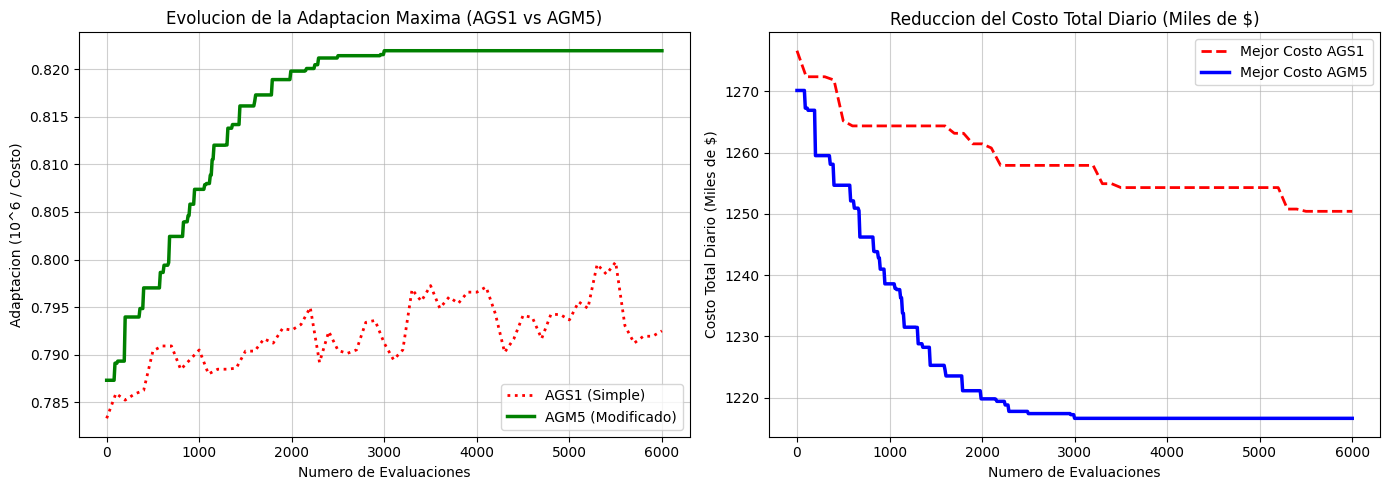
\includegraphics[width=0.95\textwidth]{output_10_1.png}%
    }{%
        \fbox{\parbox{0.9\textwidth}{\centering \vspace{1.1cm} \textit{[Colocar imagen como \texttt{output\_uc\_1.png}: Evolución de la Adaptación Máxima y Reducción del Costo Total Diario (AGS1 vs AGM5)]} \vspace{1.1cm}}}%
    }
    \caption{Evolución de la adaptación máxima y reducción del costo diario en función del número de evaluaciones (AGS1 vs AGM5).}
    \label{fig:evolucion_uc}
\end{figure}

\begin{figure}[H]
    \centering
    \IfFileExists{output_10_2.png}{%
        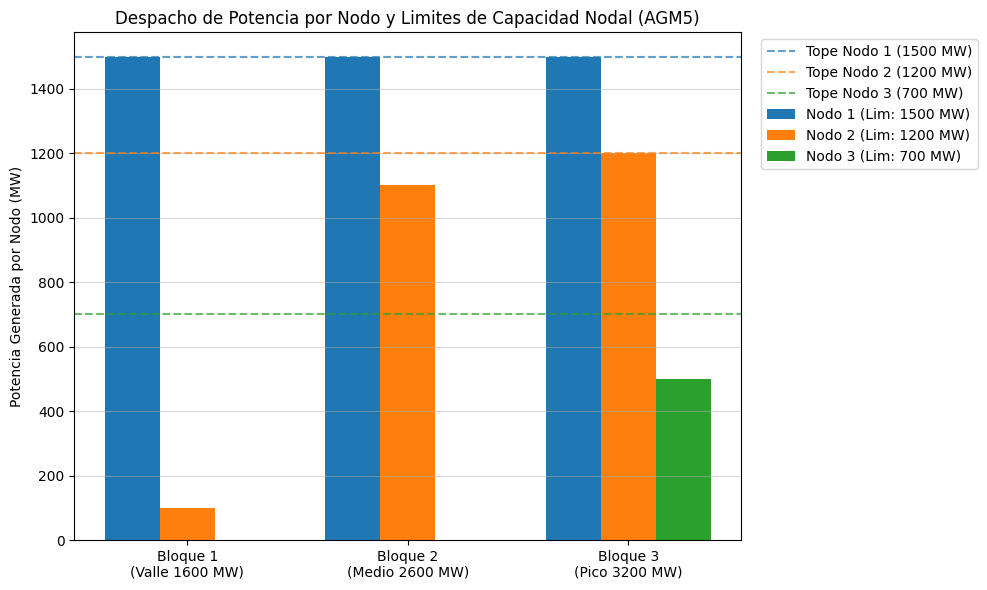
\includegraphics[width=0.85\textwidth]{output_10_2.png}%
    }{%
        \fbox{\parbox{0.9\textwidth}{\centering \vspace{1.1cm} \textit{[Colocar imagen como \texttt{output\_uc\_2.png}: Despacho de Potencia por Nodo y Límites de Capacidad Nodal (AGM5)]} \vspace{1.1cm}}}%
    }
    \caption{Potencia despachada por nodo en cada bloque horario frente a los límites máximos de transmisión.}
    \label{fig:barras_nodos}
\end{figure}

A partir de los resultados obtenidos en las Tablas \ref{tab:despacho_20_unidades}, \ref{tab:resumen_nodos_lambda} y \ref{tab:resumen_economico} y en las Figuras \ref{fig:evolucion_uc} y \ref{fig:barras_nodos}, se observa lo siguiente:
\begin{itemize}
    \item \textbf{Efecto de la congestión en el Nodo A y separación de costos incrementales ($\lambda$):} En la Tabla \ref{tab:despacho_20_unidades} se observa que las cuatro unidades de base del Nodo A (G1, G2, G3 y G4), que ya se encontraban encendidas en $t=0$, suman una capacidad de $1550\text{ MW}$. Debido al límite de transmisión de $1500\text{ MW}$ del Nodo A, el algoritmo mantiene encendidas únicamente estas cuatro máquinas durante todo el día (G1, G2 y G3 a plena carga y G4 en $250\text{ MW}$) con un costo incremental local de $\lambda_A = 19.05\text{ \$/MWh}$, sin encender nunca a G5, G6 ni G7 porque su potencia no podría salir del nodo.
    \item \textbf{Escalamiento de generación entre los Bloques Valle, Medio y Pico:} En el Bloque 1 ($1600\text{ MW}$), una vez que el Nodo A aporta sus $1500\text{ MW}$ máximos, el AGM5 enciende únicamente a la máquina más económica del Nodo B (G8 con $100\text{ MW}$ y $\lambda_B = 20.10\text{ \$/MWh}$). En el Bloque 2 ($2600\text{ MW}$), el Nodo B absorbe los $1100\text{ MW}$ faltantes encendiendo de G8 a G11, manteniendo apagado todo el Nodo C. Finalmente, en el Bloque 3 ($3200\text{ MW}$), tanto el Nodo A ($1500\text{ MW}$) como el Nodo B ($1200\text{ MW}$) llegan al tope de sus líneas de transmisión, obligando a encender las unidades G15, G16, G17 y G18 del Nodo C para generar los $500\text{ MW}$ restantes a un costo incremental de $\lambda_C = 29.84\text{ \$/MWh}$.
    \item \textbf{Ahorro económico del AGM5 y costo de la congestión de red:} Como se aprecia en la Tabla \ref{tab:resumen_economico}, el AGM5 logró reducir el costo operativo diario en $\$34\,728.40$ respecto al AGS1 ($1\,148\,342.10\text{ \$}$ frente a $1\,183\,070.50\text{ \$}$), ya que el AGS1 deja encendidas turbinas innecesarias que incrementan tanto el gasto en vacío ($\alpha_i$) como los arranques. Por otra parte, al comparar el caso con límites nodales frente al caso ideal sin restricciones de red ($1\,100\,780.40\text{ \$}$), se determina que los cuellos de botella en las líneas de transmisión de los Nodos A y B representan un sobrecosto diario de $\$47\,561.70$ por no poder aprovechar los $700\text{ MW}$ adicionales de generación barata instalados en el Nodo A.
\end{itemize}

\section{Conclusiones}

\begin{enumerate}
    \item La combinación del Algoritmo Genético Modificado (AGM5) para decidir el estado binario de encendido y apagado ($U_{i,t}$) con el método del costo incremental ($\lambda$) para repartir la potencia continua ($P_{i,t}$) permitió resolver de forma rápida y exacta el despacho de las $20$ máquinas generadoras, asegurando el cumplimiento del balance de demanda en los tres bloques horarios.
    \item Las limitaciones de potencia máxima en los nodos modifican directamente los valores de $\lambda$ del sistema: cuando los Nodos A y B alcanzan sus límites de $1500\text{ MW}$ y $1200\text{ MW}$ en hora pico, el sistema deja de tener un único $\lambda$ global y presenta tres costos incrementales distintos ($\lambda_A = 19.05$, $\lambda_B = 23.36$ y $\lambda_C = 29.84\text{ \$/MWh}$).
    \item El algoritmo AGM5 superó ampliamente al algoritmo simple AGS1 tanto en velocidad de convergencia como en ahorro económico diario, evitando arranques innecesarios de unidades de pico y encontrando la combinación exacta de máquinas que minimiza el costo total de operación.
\end{enumerate}

\end{document}